\documentclass[11pt,dvipsnames]{beamer}
\usetheme{default} 

\setbeamertemplate{navigation symbols}{} %gets rid of navigation symbols
\setbeamertemplate{footline}{} %gets rid of bottom navigation bars
\setbeamertemplate{footline}[page number]{} %use this for page numbers

\setbeamertemplate{footline}{%
  \raisebox{5pt}{\makebox[\paperwidth]{\hfill\makebox[10pt]{\scriptsize\insertframenumber~~}}}}

\setbeamertemplate{itemize items}[circle] %round bullet points
\setlength\parskip{10pt} % white space between paragraphs

\usepackage{wrapfig}
\usepackage{subfig}
\usepackage{setspace}
\usepackage{enumerate}
\usepackage{graphicx}
\usepackage{amsmath}
\usepackage{amsfonts}
\usepackage{amssymb}
\usepackage{amsthm}
\usepackage[UKenglish]{isodate}
\usepackage{tikz}
\usepackage{pgfplots}
\usepackage{natbib}
\def\checkmark{\tikz\fill[scale=0.4](0,.35) -- (.25,0) -- (1,.7) -- (.25,.15) -- cycle;} 

% allow drawing arrows
\usetikzlibrary{arrows}
\tikzstyle{arrow}=[draw, -latex] 

% bracketing shortcuts
\newcommand{\paren}[1]{\left(#1\right)}
\newcommand{\sqbracket}[1]{\left[#1\right]}
\newcommand{\cbracket}[1]{\left\{#1\right\}}
\newcommand{\abs}[1]{\left\lvert#1\right\rvert}
\newcommand{\norm}[1]{\left\lVert#1\right\rVert}
% set up the argmin operator, argmax
\DeclareMathOperator*{\argmin}{arg\,min}
\DeclareMathOperator*{\argmax}{arg\,max}

\newcommand{\myframe}[1]{\begin{frame} \frametitle{#1}}
% New itemize environment, with spaces
\newenvironment{spaceitemize}
{ \begin{itemize}
    \setlength{\itemsep}{10pt}
    \setlength{\parskip}{0pt}
    \setlength{\parsep}{0pt}     }
{ \end{itemize}                  } 


% the preamble
\title{Day 1, Session 1: Order of operations and negative numbers}
\author{Brian D. Williamson}
\institute{EPI/BIOST Bootcamp 2018}
\date{21 September 2018}

% Start the document
\begin{document}
% The title page
\begin{frame}
\titlepage
\end{frame}

\begin{frame}
\frametitle{Learning objectives}
By the end of this session, you should be able to
\begin{itemize}
\item \textbf{use} the order of operations to answer public health questions
\item \textbf{determine} the relative ordering of two numbers
\item \textbf{use} \textcolor{ForestGreen}{algebra} and \textcolor{cyan}{fractions} to answer public health questions
\end{itemize}
\end{frame}

\section{Teaser: word problems}
\myframe{Example: kidney stones \small(from Katie Kerr's BIOST 514, Autumn 2014)}
A study compared the success rates of two different procedures for removing kidney stones:  open surgery (OS) and percutaneous nephrolithotomy (PCNL), a minimally invasive technique.  Here are the numbers of procedures that were successful or not at getting rid of patients' kidney stones, by type of procedure.  The data are separated by patients with small kidney stones and large kidney stones.

{\scriptsize
\centering
Patients with Small Stones: \hspace{0.5cm} Patients with Large Stones: 

\hspace{1.3cm}
\begin{tabular}{lcc}
 & OS & PCNL \\
 \hline
 Success & 81 & 234 \\
 Failure & 6 & 36 \\
 \hline
\end{tabular}
\hspace{1cm}
\begin{tabular}{lcc}
 & OS & PCNL \\
 \hline
 S & 192 & 55 \\
 F & 71 & 25 \\
 \hline
\end{tabular}
}

\end{frame}

\myframe{Example: kidney stones}
Combined data:
\begin{tabular}{lcc}
 & OS & PCNL \\
 \hline
 S & 273 & 289 \\
 F & 77 & 61 \\
 \hline
\end{tabular}

We can ask a few questions using these data:
\begin{spaceitemize}
\item What is the \textcolor{green}{percentage} of kidney stones successfully removed for each procedure? \pause
\item What is the percentage of \textcolor{purple}{small kidney stones} successfully removed? The percentage of \textcolor{purple}{large kidney stones}?  \textcolor{cyan}{Which type of stones seem easier to treat}? \pause
\item What is the percentage of successful procedures of each type for small kidney stones only, and for large stones only?
\end{spaceitemize}
\end{frame}

\myframe{Example: kidney stones}
To solve these questions, we will need a variety of tools: \pause
\begin{spaceitemize}
\item \textcolor{green}{fraction manipulation}: percentages are fractions! \pause
\item \textcolor{blue}{the order of operations}: make sure that we get correct denominators for the fractions \pause
\item \textcolor{purple}{reading 2x2 tables}: get the correct numbers for each question \pause
\item \textcolor{cyan}{parsing sentences}: which information is relevant?
\end{spaceitemize}

We will cover each of these tools in more detail!
\end{frame}

\myframe{Example: statistics in medical research \small (from Katie Kerr's BIOST 514, Autumn 2014)}
Does involving a statistician to help with statistical methods improve the chance that a medical research paper will be published?  \pause

A study of a random sample of papers submitted to two medical journals found that 135 of 190 papers that lacked statistical assistance were rejected by the journal editors (without even being circulated for peer review).  In contrast 293 of the 514 papers with statistical help were rejected without review.  \pause

(Note:  a paper is ``submitted'' when it is sent to a journal for consideration for publication.  Not all submitted papers are accepted by the journal editors and published in the journal.)

\end{frame}

\myframe{Example: statistics in medical research}
To find out if involving a statistician helps: \pause
\begin{spaceitemize}
\item Determine the \textcolor{green}{proportion} of papers submitted to these journals that include help from a statistician. \pause
\item Give a 95\% \textcolor{cyan}{confidence interval (CI)} for this proportion, and \textcolor{cyan}{interpret it}. \pause
\item Determine the \textcolor{green}{proportion} of papers rejected without review when a \textcolor{purple}{statistician is and is not involved}. \pause
\item Give a 95\% CI for this proportion, and interpret it. \pause
\item Is this an \textcolor{purple}{observational study or a randomized trial}? \pause
\item Write a paragraph summarizing the conclusions of your analysis, making sure to comment on the ability of the study to address the question of interest and on any important limitations of the study.
\end{spaceitemize}
\end{frame}

\myframe{Example: statistics in medical research}
These questions also involve a variety of tools:
\begin{spaceitemize}
\item \textcolor{green}{fraction manipulation}
\item \textcolor{purple}{parsing sentences}
\item \textcolor{cyan}{interpreting results}
\end{spaceitemize}
\end{frame}

\myframe{Outline for Session 1}
\begin{spaceitemize}
\item Order of operations
\item Negative numbers 
\item Fractions
\item Algebra
\end{spaceitemize}
\end{frame}

\section{Order of operations}
\myframe{Evaluating expressions}\label{ex:oo1}
\begin{itemize}
\item Example expression: $3(1 + 2) + 5$
\item[]
\item How do we evaluate the above expression? In other words: \pause
\begin{itemize}
\item Which terms to we compute first?
\item[] \pause
\item Are there rules for evaluating expressions?
\end{itemize}
\end{itemize}
\end{frame}

\myframe{Order of operations}
\begin{itemize}
\item Rules for evaluating expressions:
\begin{enumerate}
\item Parentheses
\item Exponents
\item Multiplication and division (\textcolor{red}{evaluate left to right})
\item Addition and subtraction (\textcolor{red}{evaluate left to right})
\end{enumerate}
\item[] \pause
\item A handy memory device: PEMDAS -- Please Excuse My Dear Aunt Sally
\end{itemize}
\end{frame}

\myframe{Example: order of operations in action!}
\begin{itemize}
\item Example from slide \ref{ex:oo1}: $3(1 + 2) + 5$
\item[]
\item This notation is equivalent to $3\times (1+2) + 5$
\item[] \pause
\item Apply PEMDAS: \hfill \underline{Current Expression}
\begin{enumerate}
\item Parentheses: add 1 and 2 \hfill $3(3) + 5$ \pause
\item Exponents: none \hfill $3(3) + 5$ \pause
\item Multiplication: multiply 3 and 3 \hfill $9 + 5$ \pause
\item Division: none \hfill $9 + 5$ \pause
\item Addition: add 9 and 5 \hfill 14 \pause
\item Subtraction: none \pause
\end{enumerate}
\item[]
\item The final answer is 14!
\end{itemize}
\end{frame}

\myframe{Example: order of operations with exponents!}
\begin{itemize}
\item Expression: $\dfrac{(2^2 + 5)^2}{3\times 3} + 5$
\item[] \pause
\item Apply PEMDAS: \hfill \underline{Current Expression} \pause
\begin{enumerate}
\item Parentheses: $2^2 + 5$. \hfill $\frac{(2^2 + 5)^2}{3\times 3} + 5$ \pause
\item[] Need to apply PEMDAS again! \pause
\begin{enumerate}
\item Parentheses: none \hfill $\frac{(2^2 + 5)^2}{3\times 3} + 5$ \pause
\item Exponents: $2^2 = 4$ \hfill $\frac{(4 + 5)^2}{3\times 3} + 5$ \pause
\item Multiplication/division: none \hfill $\frac{(4 + 5)^2}{3\times 3} + 5$ \pause
\item Addition/subtraction: $4 + 5 = 9$ \hfill $\frac{(9)^2}{3\times 3} + 5$
\end{enumerate} \pause
\item Exponents: $9^2 = 81$ \hfill $\frac{81}{3\times 3} + 5$ \pause
\item Multiplication: $3 \times 3 = 9$ \hfill $\frac{81}{9} + 5$ \pause
\item Division: $81/9 = 9$ \hfill $9 + 5$ \pause
\item Addition/subtraction: $9 + 5 = 14$!
\end{enumerate}
\end{itemize}
\end{frame}

\myframe{Order of operations: nesting}
\begin{itemize}
\item Earlier, we needed to apply PEMDAS a second time, within the evaluation of the parentheses
\item[]
\item This is common!
\item[]
\item Apply PEMDAS as many times as necessary within each sub-expression, like $(2^2 + 5)$ in the previous example
\end{itemize}
\end{frame}

\myframe{Exercise: order of operations}
Kidney stone data:

{\scriptsize
Patients with Small Stones: \hspace{0.5cm} Patients with Large Stones: \hspace{0.5cm} Combined data:

\hspace{-0.4cm}
\begin{tabular}{lcc}
 & OS & PCNL \\
 \hline
 Success & 81 & 234 \\
 Failure & 6 & 36 \\
 \hline
\end{tabular}
\hspace{0.8cm}
\begin{tabular}{lcc}
 & OS & PCNL \\
 \hline
 S & 192 & 55 \\
 F & 71 & 25 \\
 \hline
\end{tabular}
\hspace{0.7cm}
\begin{tabular}{lcc}
 & OS & PCNL \\
 \hline
 S & 273 & 289 \\
 F & 77 & 61 \\
 \hline
\end{tabular}
}

Try to work out these examples alone or in pairs:
\begin{enumerate}
\item 273/(273+77) and 289/(289+61). What proportions do these correspond to?
\item What is the percentage of small kidney stones successfully removed? Large kidney stones?
\item Which type of kidney stones seem easier to treat?
\item PEMDAS example: $\{(2+1)^2 + 1\}^2$ 
\end{enumerate}
\end{frame}

%\myframe{Solution: order of operations}
%\begin{enumerate}
%\item These correspond to the proportion of kidney stones successfully removed in OS and PCNL, respectively. We find the proportions using PEMDAS: \pause
%\begin{itemize}
%\item Parentheses: $273+77 = 350$ \pause
%\item Division: $273/350 = 0.78$, or 78\% (OS)
%\item Parentheses: $289+61 = 350$ \pause
%\item Division: $289/350 = 0.82$, or 82\% (PCNL)
%\end{itemize}
%\item[] \pause
%\item We first have to find the numbers of small and large kidney stones successfully removed, and then find the total number of both small and large kidney stones operated on. \pause
%\begin{itemize}
%\item Small kidney stones removed: $81+234$; Large: $192+55$ \pause
%\item Total small stones operated on: $81+234+6+36$; Large: $192+55+71+25$ \pause
%\item Proportion small: $(81+234)/(81+234+6+36) = 315/357 \approx 0.88$, or 88\% \pause
%\item Proportion large: $(192+55)/(192+55+71+25) = 247/343 \approx 0.72$, or 72\% \pause
%\end{itemize}
%\end{enumerate}
%\end{frame}
%
%\myframe{Solution: order of operations}
%\begin{enumerate}
%\item[3.] Based on the numbers calculated in (1) and (2), it seems that small kidney stones are easier to treat. \pause
%\item[]
%\item[4.] $\{(2+1)^2 + 1\}^2 = 100$. PEMDAS: \pause
%\begin{itemize}
%\item Parentheses: $(2 + 1)^2 + 1$. Nested PEMDAS:
%\begin{itemize}
%\item Parentheses: $2 + 1$. Nested PEMDAS -- Addition: $2 + 1 = 3$
%\item Exponent: $3^2 = 9$ 
%\item Addition: $9 + 1 = 10$
%\end{itemize} \pause
%\item Exponent: $10^2 = 100$
%\end{itemize}
%\end{enumerate}
%\end{frame}

\section{Negative numbers}
\myframe{Negative numbers: what are they?}
\begin{itemize}
\item Ways to think about negative numbers: \pause
\begin{itemize}
\item A positive number subtracted from zero \pause
\item[]
\item Opposites of positive numbers: $-4 + 4 = 0$ \pause
\item[]
\item Movement left on the number line \pause
\end{itemize}
\item[]
\item When might we see them? \pause
\begin{spaceitemize}
\item Comparing two proportions \pause
\item Decreasing trend (e.g., lung capacity for smokers vs. non-smokers)
\end{spaceitemize}
\end{itemize}
\end{frame}

\myframe{The number line}
\begin{itemize}
\item Movement on the number line: \pause
\begin{itemize}
\item Right (positive numbers): 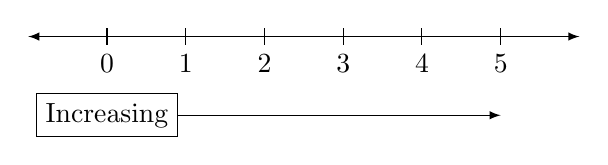
\begin{tikzpicture}
\draw[latex-latex] (-1, 0) -- (6, 0) ; %edit here for the axis
\foreach \x in  {0,1,2,3,4,5} % edit here for the vertical lines
\draw[shift={(\x,0)},color=black] (0pt,3pt) -- (0pt,-3pt);
\foreach \x in {0,1,2,3,4,5} % edit here for the numbers
\draw[shift={(\x,0)},color=black] (0pt,0pt) -- (0pt,-3pt) node[below] 
{$\x$};
\node[draw] (inc) at (0, -1) {Increasing};
\path [arrow] (inc) -- (5, -1);
\end{tikzpicture} \pause
\item[]
\item Left (negative numbers): 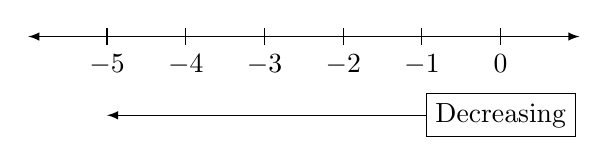
\begin{tikzpicture}
\draw[latex-latex] (-6, 0) -- (1, 0) ; %edit here for the axis
\foreach \x in  {0,-1,-2,-3,-4,-5} % edit here for the vertical lines
\draw[shift={(\x,0)},color=black] (0pt,3pt) -- (0pt,-3pt);
\foreach \x in {0,-1,-2,-3,-4,-5} % edit here for the numbers
\draw[shift={(\x,0)},color=black] (0pt,0pt) -- (0pt,-3pt) node[below] 
{$\x$};
\node[draw] (dec) at (0, -1) {Decreasing};
\path [arrow] (dec) -- (-5, -1);
\end{tikzpicture}
\end{itemize}
\item[] \pause
\item Example: move left 3, starting at 100? \pause
\begin{itemize}
\item Subtract 3 \pause
\item Add negative 3
\end{itemize}
\end{itemize}
\end{frame}

\myframe{Properties of negative numbers}
\begin{itemize}
\item Represent opposites of positive numbers, or movement left on the number line
\item[] \pause
\item Subtraction = adding a negative number
\item[] \pause
\item The product of two negatives is a positive
\item[] \pause
\item Movement left on the number line $\rightarrow$ smaller numbers
\end{itemize}
\end{frame}

\myframe{Negative fractions}
\begin{itemize}
\item First, positive fractions: for the same numerator, a larger denominator makes a smaller number, e.g., 1/4 $<$ 1/2
\item[] \pause
\item Negatives are opposites: think of zero as a mirror
\item[] \pause
\item So for the same numerator (a negative number), a larger denominator makes a less negative number, e.g., $-1/2 < -1/4 $
\end{itemize}
\end{frame}

\myframe{Example: two negatives make a positive}
\begin{itemize}
\item Expression: $-1 \times -1$
\item[] \pause
\item Answer: 1!
\item[]
\item Why? \pause
\begin{itemize}
\item $-1$ is a negative number
\item[] \pause
\item Negative numbers mean opposites; the opposite of $-1$ is 1
\end{itemize}
\end{itemize}
\end{frame}

\myframe{Example: ordering negative numbers}
\begin{itemize}
\item Expression: $-3 \ \rule{.5cm}{0.15mm} \ -2$
\item[] \pause
\item Answer: $-3 < -2$
\item[] \pause
\item Why? \pause
\begin{itemize}
\item Negative numbers are left motion on number line! -3 is further left than -2
\end{itemize}
\end{itemize}
\end{frame}

\myframe{Exercise: negative numbers}
\begin{itemize}
\item Try to work out the following examples by yourself or in pairs:
\begin{enumerate}
\item $-5.2 - (-11.3)$
\item[]
\item $-5 - 6$
\item[]
\item $(-1)\times(-5) + (-3)$
\item[]
\item $-\dfrac{3}{7} - \left(-\dfrac{1}{4}\right)$
\end{enumerate}
\end{itemize}
\end{frame}

%\myframe{Solution: negative numbers}
%\begin{enumerate}
%\item $-5.2 - (-11.3) = 6.1$ \pause
%\begin{itemize}
%\item $-(-11.3) = -1 \times (-11.3) = 11.3$ \pause
%\item $-5.2 + 11.3 = 11.3 - 5.2 = 6.1$
%\end{itemize}
%\item[] \pause
%\item $-5 - 6 = -11$
%\item[] \pause
%\item $(-1)\times(-5) + (-3) = 2$ \pause
%\begin{itemize}
%\item $-1 \times (-5) = 5$ \pause
%\item $5 + (-3) = 5 - 3 = 2$
%\end{itemize}
%\item[] \pause
%\item $-\dfrac{3}{7} - \left(-\dfrac{1}{4}\right) = -5/28 \approx -0.17$ \pause
%\begin{itemize}
%\item $-\dfrac{3}{7} - \left(-\dfrac{1}{4}\right) = \dfrac{3}{7} + \dfrac{1}{4}$ \pause
%\item $-\dfrac{3}{7} + \dfrac{1}{4} = -12/28 + 7/28 = -5/28$
%\end{itemize}
%\end{enumerate}
%\end{frame}

\myframe{Related concepts: absolute value}
\begin{itemize}
\item Magnitudes: how ``large'' is a number, with no direction
\begin{itemize}
\item Examples: speed (how fast an object is moving), length 
\end{itemize}
\item[] \pause
\item Symbol for absolute value is $|\cdot |$
\end{itemize}
\centering
\begin{tikzpicture}
        \begin{axis}[%
            domain = -1:1,
            range = -1:1,
            samples = 50,
            axis x line = center,
            axis y line = center,
            xlabel = {$x$},
            ylabel = {$y$},
            ticks = none
            ]
            \addplot[blue] {abs(x)} [yshift=3pt] node[pos=.95,left] {$y=|x|$};
        \end{axis}
    \end{tikzpicture}
\end{frame}

\myframe{Example: absolute value of a positive number}
\begin{itemize}
\item Expression: $|4|$
\item[] \pause
\item Answer is 4! Positive numbers already measure size, with no direction
\end{itemize}
\end{frame}

\myframe{Example: absolute value of a negative number}
\begin{itemize}
\item Expression: $|-4|$
\item[] \pause
\item Answer is 4!
\item[]
\item Why? \pause
\begin{itemize}
\item Negatives are opposites of positives \pause
\item Absolute value has no direction \pause
\item 4 and $-4$ are equally far away from zero
\end{itemize}
\end{itemize}
\end{frame}

\myframe{Related concepts: negative numbers and inequalities}
\begin{itemize}
\item Expression from before: $-3 < -2$ \pause
\item[]
\item What happens if we multiply both sides by $-1$?
\item[] \pause
\item Negatives are opposites: signs change and inequality flips, yielding $2 < 3$
\end{itemize}
\end{frame}

\myframe{Back to negative fractions}
\begin{itemize}
\item Recall that for a fixed negative numerator, a larger denominator means a less negative number 
\item[] \pause
\item Absolute value makes this more clear!
\item[] \pause
\item Example: $-1/2$, $-1/4$ \pause
\begin{enumerate}
\item $|-1/2| = 1/2$, $|-1/4| = 1/4$
\item[] \pause
\item We already know that $1/4 < 1/2$
\item[] \pause
\item Multiply both sides by $-1$, yielding (with inequality rules) $-1/2 < -1/4$
\end{enumerate}
\end{itemize}
\end{frame}

\myframe{Exercise: absolute value, negative numbers}
\begin{itemize}
\item Try to work out the following examples by yourself or in pairs:
\begin{enumerate}
\item $|-5|$ and $|5|$
\item[]
\item Is $|-5| < 4$?
\item[]
\item Is $-15 > -14$? 
\item[]
\item Is $-(3 + 1)\times 5 < -(4 + 1)\times 3$?
\end{enumerate}
\end{itemize}
\end{frame}

%\myframe{Solution: absolute value, negative numbers}
%\begin{enumerate}
%\item $|-5| = |5| = 5$
%\item[]
%\item $|-5| = 5$, and $5 > 4$; answer is no
%\item[]
%\item $-15$ is further from 0 than $-14$; also, 14 $<$ 15. Hence $-15 < -14$
%\item[]
%\item (at least) Two ways to solve this: \pause
%\begin{itemize}
%\item $-(3+1)\times 5 = -1\times(4)\times 5 = -20$, and $-(4+1)\times 3 = -1\times (5) \times 3 = -15$. So $-20 < -15$
%\item[] \pause
%\item If $-(3+1)\times 5 < -(4+1)\times 3$, then $(3+1)\times 5 > (4+1)\times 3$. But this means $20 > 15$, which is true!
%\end{itemize}
%\end{enumerate}
%\end{frame}

\myframe{Summary}
\begin{itemize}
\item Solving word problems requires a variety of tools: \textcolor{green}{fraction manipulation}, \textcolor{purple}{parsing text}, \textcolor{blue}{the order of operations}, \textcolor{red}{negative numbers}, and \textcolor{cyan}{interpreting results}, among others
\item[] \pause
\item The order of operations is a recipe for solving expressions
\item[] \pause
\item A handy memory tool is PEMDAS: Parentheses, Exponents, Multiplication/Division, Addition/Subtraction
\item[] \pause
\item Negative numbers decrease as we move away from zero (left on the number line)
\item[] \pause
\item Absolute value measures the magnitude of a number -- how far away from zero is it?
\item[]
\end{itemize}
\end{frame}
\end{document}
